\chapter{Energy Conversion}
\label{ch:conv}

Energy and power take many different forms, from the initial sources to the end results used. Necessarily, methods have been developed to convert the different forms of energy or power from one to another. The first method addressed in this chapter is the conversion process of thermal to mechanical to electrical energy found in heat engines and generators. This thesis is focused on geothermal heat, however heat engines can be used with a number of different sources including the burning of a fuel such as biomass or coal, or even as waste heat from an independent process. Next conversion between different forms of electrical power will be addressed.

%This file used to contain the geothermal chapter, now contains thermal/mechanical section of the conversion chapter
\section{Thermal Energy}
Thermal energy, or heat, can originate from many different sources including combustion of a fuel, radioactive decay, or absorption of light from the sun. Heat can be used directly to warm a building, but it is also a critical step in most traditional methods of generating electrical power. 
%\chapter{Geothermal Energy}
%\label{ch:geothermal}

\subsection{Enthalpy}
Enthalpy describes the energy of a system available to be converted to work. It is related to the temperature of the geothermal resource, but also dependent on the pressure and volume. Temperature is usually the primary metric of a resource, but even a high temperature source is useless without sufficient volume flow. Quantitatively enthalpy is expressed as \cite{Nellis2009}
\begin{equation}
H = U + pV
\end{equation}
where $U$ is the internal energy, which is function of temperature, $p$ is the pressure of the system, and $V$ is the volume. Generally it is more convenient to use the change in enthalpy rather than absolute values. After a system undergoes some thermodynamic process, the system will always have some remaining internal energy, pressure, and volume. Therefore, a change in enthalpy better describes the energy extracted from (or absorbed by) the system.
Additionally, the enthalpy of a system is often normalized by the its mass for comparison to other sized systems and the mass specific enthalpy, $h$, is used instead.
\nomenclature[V]{$H$}{Enthalpy of a fluid\nomunit{\si{\joule}}}
\nomenclature[V]{$U$}{Internal energy of a fluid\nomunit{\si{\joule}}}
\nomenclature[V]{$p$}{Aboluete fluid pressure\nomunit{\si{\pascal}}}
\nomenclature[V]{$V$}{Fluid volume\nomunit{\si{\meter\cubed}}}
\nomenclature[V]{$h$}{Mass specific enthalpy of a fluid\nomunit{\si{\joule\per\kilogram}}}


\subsection{Geothermal Cycles}
%%Describe each of the following but focus on cycles for low enthalpy sources
Geothermal systems can be classified as high-, medium-, or low-enthalpy\footnote{While the technical definitions differ, the terms enthalpy, heat, and temperature are often used interchangeably when qualitatively describing geothermal sources.}. Although there is no formal delineation, high-enthalpy sources generally have temperatures greater than about $150$ \textcelsius{} ($302$ \textdegree{}F) and low-enthalpy sources have temperatures lower than $100$ \textcelsius{} ($212$ \textdegree{}F) \cite{Norden2011}. Depending on the amount of extractable energy of the resource, different geothermal processes or cycles can be used to extract the maximum amount of energy from the resource.

\subsubsection{Dry Steam}
This high-enthalpy processes extracts hot steam from the earth. The steam is sent directly through a turbine then condensed into liquid water and injected back underground. 

\subsubsection{Flash Steam} 
In the flash steam process high pressure hot water is extracted then, allowed to boil becoming steam and low pressure hot water. The steam is sent through a turbine then condensed, recombined with water, and injected back underground.

\subsubsection{Binary Cycle} 
As the name implies, binary cycles involve two loops: a heat source loop and working fluid loop. Heat is collected in the heat source loop and transferred to the working loop through a heat exchanger. The working fluid then undergoes the vaporization process to spin a turbine or other type of expander. The expander is connected to a generator which converts the rotational mechanical energy into electrical energy. After some of the heat is converted, the working fluid passes through a condenser where it is cooled further. Sometimes the cooling process involves drawing in air at ambient temperature, but it can also involve a third loop. The fluids within each of the cycles must be moved using pumps. The pumps themselves need to be powered and act as a parasitic load to the system.

Binary cycles are not limited to low or medium enthalpy heat sources. The most common binary cycle is the Rankine Cycle. A diagram of the process can be seen in \autoref{fig:rankine_cycle_diagram}. In an ideal Rankine Cycle heat is added to the working fluid under high pressure to change its phase from liquid to gas. The fluid expands isentropically\footnote{In thermodynamics, isentropic processes do not have a net change in entropy.} which rotates the generator shaft, causing the fluid's temperature and pressure to drop. Additional heat is then expelled from the fluid as it condenses at a constant low pressure side of the system. Finally the fluid is isentropically pumped back to the high pressure and the process begins again.
\begin{figure}[h]
	\centering

	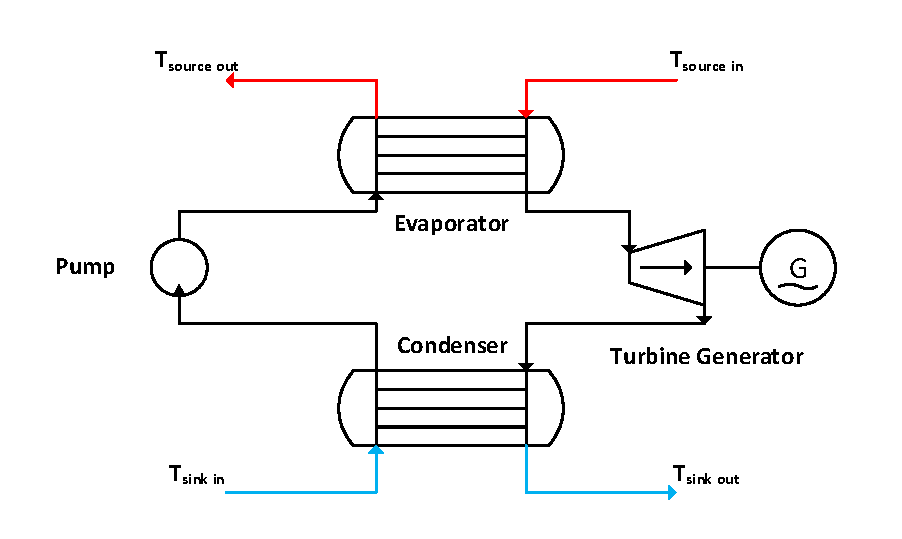
\includegraphics[width=\textwidth]{figures/RankineCycleDiagram.pdf}

	\caption{Diagram of a Rankine cycle system.}
	\label{fig:rankine_cycle_diagram}
	
\end{figure}

For geothermal sources, generally high enthalpy systems can be implemented directly with a single loop using the flash or dry steam processes. However, for lower enthalpy systems, water cannot be used as a working fluid because the temperatures are not high enough to vaporize it. In these cases an organic Rankine cycle, which uses an organic working fluid such as refrigerants instead of water, can be employed. Working fluids are typically selected for relatively low vaporization temperatures, but the thermodynamic states of the heat source must also be considered. The selection of the type of expander and pumps are discussed in Kreider \cite{Kreider}. Generally larger diameter expanders operate at lower speeds.




%\subsection{Pilgrim Hot Springs}
%Do this in 1st chapter not conv/geotherm chapter
%More thourough description of the resource and potential development plans.

 %used to contain geothermal chapter, now contains thermal section


\section{Electrical Generators}
%This section should focus the difference between the two with respect to geothermal sources. I can have a fundemental description of the generators either in this chapter or the intro chapter.
Electrical generators are spinning machines which convert the mechanical power of rotating a shaft to electrical power. Fundamentally, they operate on the principles of Maxwell's and Faraday's laws which broadly state that a moving magnetic field produces an electric field and vice versa. The primary difference among generator types is how that magnetic is produced. 
%As previously described, asynchronous generators, also called induction generators, are incapable maintaining a grid. Synchronous generators supply or absorb reactive power depending on the needs of the grid.

\subsection{Synchronous Generators}
The magnetic fields of Synchronous generators are formed by external sources. The name derives from the fact that electric frequency directly synchronizes with the physical rotation of the machine.\footnote{Certain wiring configurations add additional electromagnetic poles to machine which causes the mechanical speed to be slower than the electrical speed by a factor of the integer number of poles.} They are capable of supplying reactive power as well as their loads because the internal magnetic field is not self induced. 

In traditional synchronous machines an electro-magnet is used to generate the field by running a DC current through the rotor windings. The spinning DC electric field produces a magnetic field, which in turn makes an electric field in the stator. By varying the DC current applied to the rotor, the user can control voltage generated by the machine. The current sets the magnetic flux, which in turn controls the voltage. \cite{Chapman2005} As discussed in \autoref{sec:droop}, droop control takes advantage of the relationship between voltage and reactive power to ensure they are appropriately balanced.

Permanent magnets are also used to form the magnetic field of the rotor. A benefit of using permanent magnets over electro-magnets is the lack of slip rings or brushes used to apply the DC current. These components can introduce a source of friction and wear down over time. However, the since permanent magnetic fields are fixed at the time of construction, the user cannot control the voltage of the machine.

\subsection{Asynchronous Generators}
Asynchronous machines generate their internal magnetic fields by self-induction rather than from an external source. Since they do not rely on an additional source or expensive material to operate, induction machines are generally have simpler designs and are more affordable than synchronous machines. However, that also means they need to consume reactive power from the grid in order to maintain their magnetic field. This field relies on a difference in frequency between the rotor and stator fields. The relative difference is represented by the machine's slip. When the slip is positive, the field frequency in the stator is greater than in the rotor\footnote{After accounting for the number of poles}, and the machine operates as a motor. A negative slip means the rotor is spinning faster than the frequency of the stator and the machine is acting as a generator. 


Some work has been done on self-excited induction generators\cite{Ouazenne1983, Ammasaigounden1986}. Instead of consuming it from the grid, these machines use a bank of capacitors connected at their leads supply the necessary reactive power in order to maintain their magnetic fields. However, a significant drawback to these devices is the lack of control over frequency and voltage.\cite{Bansal2005} For this they have not seen commercial implementation, and if they do it will likely be limited to isolated systems.

\section{Electronic Conversion}
As described previously, electronic conversion takes electric power from either an AC or DC form and converts it to a different form or level. This is generally done by switching the path of the input current to form the desired output. Control over the switching is critical for these conversion devices. Pulse Width Modulation (PWM) and Pulse Frequency Modulation (PFM) are two alternate methods of controlling switching states of the semiconductor devices. Both methods vary the duty cycle\footnote{The fractional time the device is on relative to one period.} of the control signal of the device in order to change the on/off state. For PWM the switching frequency is held constant while the duration of the pulse is varied to control the output. In PFM, the duration of each pulse is fixed while time between pulses, and therefore the frequency, does vary.
%\subsection{Linear Power Supplies}
%Linear

%\subsection{Switched Mode Power Supplies}

\subsection{DC-DC}
%description, diagram, and waveform of simple buck and boost converters
DC-DC power conversion devices can generally be divided up into two simple designs: buck to step voltage down and boost to step voltage up. The concepts used in these two designs can be modified or combined to create a number of  DC-DC converter topologies with slightly different characteristics. These include but are not limited to \'Cuk, SEPIC, Flyback, Forward, Half-bridge, and Full-bridge converters. \cite{Mohan2003}

In a simple Buck converter, seen in \autoref{fig:simple_buck}, timed switching sets the average output voltage to a value smaller than the input. The inductor ensures a continuous current at the output and the capacitor provides a steady voltage with only modest ripple. 
%Example waveforms of input and output current and voltage can be seen for a simple buck converter in fig X.

\begin{figure}[h]
	
\centering


\begin{tikzpicture}[american voltages]
\draw[color=black, thick]
%Input
(0,0) to [V, l=$V_{in}$, invert] (0,3){}

%high 
(3,3) to [L] (6,3) -- (7,3){}

%switch
(0,3) to [Tnmos] (3,3) {}

%Diode
(3,0) to [D*, *-*] (3,3){}

%low
(0,0) -- (7,0){}

%output
(7,3) to [open, l=$V_{out}$, o-o] (7,0){}
(6,3) to [C, *-*] (6,0){}
;
\end{tikzpicture}
\caption{Simplified diagram of a buck converter.}
\label{fig:simple_buck}

\end{figure}

In a simple Boost converter, seen in \autoref{fig:simple_boost}, timed switching also sets the average output voltage to the desire level. However, the placement of the components leads to an increasing current through the inductor while the switch is closed. When the switch is open, the relatively high current flow through the diode and results in a larger average output voltage than seen at the input. As in the buck converter, the capacitor provides a steady voltage. 
%Example waveforms of input and output current and voltage can be seen for a simple buck converter in fig X.

\begin{figure}[h]
	
\centering

\begin{tikzpicture}[american voltages]
\draw[color=black, thick]
%Input
(0,0) to [V, l=$V_{in}$, invert] (0,3){}

%high 
(0,3) to [L] (3,3) to [D*] (6,3) -- (7,3){}

%switch
(3,1.5) node[nmos] (mos) {}
(mos.gate) node[anchor=east] {}
(mos.drain) to [short, -*] (3,3){}
(mos.source) to [short, -*] (3,0){}

%low
(0,0) -- (7,0){}

%output
(7,3) to [open, l=$V_{out}$, o-o] (7,0){}
(6,3) to [C, *-*] (6,0){}
;
\end{tikzpicture}
\caption{Simplified diagram of a boost converter.}
\label{fig:simple_boost}


\end{figure}

\subsection{Rectifier and Inverter}
%description, diagram, and waveform of simple rectifier
Simple rectifiers use a combination of diodes to convert an AC voltage to DC. \autoref{fig:simple_rectifier} shows a simple example of a single phase rectifier. The diodes allow a path such that the DC current always flows in the same direction regardless of AC polarity. More advance designs will use active switching devices and a control scheme to provide the same function. Though more complicated to implement, the user has more direct control over the output as well as how the load appears to the input. 
%Example waveforms of input and output current and voltage can be seen for a simple buck converter in fig X.

\begin{figure}[h]
	
\centering
\caption{Simplified diagram of a single phase full-bridge rectifier.}
\label{fig:simple_rectifier}


\begin{tikzpicture}
\draw[color=black, thick]
% AC leads
%(0,1) to [short] (4,1) to [short] (4,2){} 
(0,1) -- (4,1) -- (4,2){} 
(0,1) to [sV, l=$v_{ac}$] (0,7) -- (4,7) -- (4,6){}

%Rectifier Diode Bridge
(2,4) to [D*, *-*] (4,6) to [D*, *-*] (6,4){}
(2,4) to [D*, *-*] (4,2) to [D*, *-*] (6,4){}

%DC leads
(2,4) -- (1,4) -- (1,0) to [short, -o] (9,0){}
(6,4) to [short, -o] (9,4){}

%Output 
(7,4) to [C, *-*] (7,0){}
(9,4) to [open, l=$v_{dc}$] (9,0)
;
\end{tikzpicture}

\end{figure}


%\subsection{Inverter}
%description, diagram, and waveform of simple inverter
Inverters function as rectifiers in reverse. A DC source is switched on and off such that it alternates periodically. In fact many inverters are designed to be reversible. The device can control the flow of active and reactive power flow in an inverter mode or a rectifier mode.

